% --- LaTeX Homework Template - S. Venkatraman ---

% --- Set document class and font size ---

\documentclass[letterpaper, 11pt]{article}

% --- Package imports ---

\usepackage{
  amsmath, amsthm, amssymb, mathtools, dsfont,	  % Math typesetting
  graphicx, wrapfig, subfig, float,                  % Figures and graphics formatting
  listings, color, inconsolata, pythonhighlight,     % Code formatting
  fancyhdr, sectsty, hyperref, enumerate, enumitem } % Headers/footers, section fonts, links, lists
\usepackage{booktabs, array, colortbl}
\usepackage{algorithm, algpseudocode}

% --- Page layout settings ---
\usepackage{bm}
% Set page margins
\usepackage[left=1.35in, right=1.35in, bottom=1in, top=1.1in, headsep=0.2in]{geometry}

% Anchor footnotes to the bottom of the page
\usepackage[bottom]{footmisc}

% Set line spacing
\renewcommand{\baselinestretch}{1.2}

% Set spacing between paragraphs
\setlength{\parskip}{1.5mm}

% Allow multi-line equations to break onto the next page
\allowdisplaybreaks

% Enumerated lists: make numbers flush left, with parentheses around them
\setlist[enumerate]{wide=0pt, leftmargin=21pt, labelwidth=0pt, align=left}
\setenumerate[1]{label={(\arabic*)}}

% --- Page formatting settings ---

% Set link colors for labeled items (blue) and citations (red)
\hypersetup{colorlinks=true, linkcolor=blue, citecolor=red}

% Make reference section title font smaller
\renewcommand{\refname}{\large\bf{References}}

% --- Settings for printing computer code ---

% Define colors for green text (comments), grey text (line numbers),
% and green frame around code
\definecolor{greenText}{rgb}{0.5, 0.7, 0.5}
\definecolor{greyText}{rgb}{0.5, 0.5, 0.5}
\definecolor{codeFrame}{rgb}{0.5, 0.7, 0.5}

% Define code settings
\lstdefinestyle{code} {
  frame=single, rulecolor=\color{codeFrame},            % Include a green frame around the code
  numbers=left,                                         % Include line numbers
  numbersep=8pt,                                        % Add space between line numbers and frame
  numberstyle=\tiny\color{greyText},                    % Line number font size (tiny) and color (grey)
  commentstyle=\color{greenText},                       % Put comments in green text
  basicstyle=\linespread{1.1}\ttfamily\footnotesize,    % Set code line spacing
  keywordstyle=\ttfamily\footnotesize,                  % No special formatting for keywords
  showstringspaces=false,                               % No marks for spaces
  xleftmargin=1.95em,                                   % Align code frame with main text
  framexleftmargin=1.6em,                               % Extend frame left margin to include line numbers
  breaklines=true,                                      % Wrap long lines of code
  postbreak=\mbox{\textcolor{greenText}{$\hookrightarrow$}\space} % Mark wrapped lines with an arrow
}

% Set all code listings to be styled with the above settings
\lstset{style=code}

% --- Math/Statistics commands ---

% Add a reference number to a single line of a multi-line equation
% Usage: "\numberthis\label{labelNameHere}" in an align or gather environment
\newcommand\numberthis{\addtocounter{equation}{1}\tag{\theequation}}

% Shortcut for bold text in math mode, e.g. $\b{X}$
\let\b\mathbf

% Shortcut for bold Greek letters, e.g. $\bg{\beta}$
\let\bg\boldsymbol

% Shortcut for calligraphic script, e.g. %\mc{M}$
\let\mc\mathcal

% \mathscr{(letter here)} is sometimes used to denote vector spaces
\usepackage[mathscr]{euscript}

% Convergence: right arrow with optional text on top
% E.g. $\converge[w]$ for weak convergence
\newcommand{\converge}[1][]{\xrightarrow{#1}}

% Normal distribution: arguments are the mean and variance
% E.g. $\normal{\mu}{\sigma}$
\newcommand{\normal}[2]{\mathcal{N}\left(#1,#2\right)}

% Uniform distribution: arguments are the left and right endpoints
% E.g. $\unif{0}{1}$
\newcommand{\unif}[2]{\text{Uniform}(#1,#2)}

% Independent and identically distributed random variables
% E.g. $ X_1,...,X_n \iid \normal{0}{1}$
\newcommand{\iid}{\stackrel{\smash{\text{iid}}}{\sim}}

% Equality: equals sign with optional text on top
% E.g. $X \equals[d] Y$ for equality in distribution
\newcommand{\equals}[1][]{\stackrel{\smash{#1}}{=}}

% Math mode symbols for common sets and spaces. Example usage: $\R$
\newcommand{\R}{\mathbb{R}}   % Real numbers
\newcommand{\C}{\mathbb{C}}   % Complex numbers
\newcommand{\Q}{\mathbb{Q}}   % Rational numbers
\newcommand{\Z}{\mathbb{Z}}   % Integers
\newcommand{\N}{\mathbb{N}}   % Natural numbers
\newcommand{\F}{\mathcal{F}}  % Calligraphic F for a sigma algebra
\newcommand{\El}{\mathcal{L}} % Calligraphic L, e.g. for L^p spaces

% Math mode symbols for probability
\newcommand{\pr}{\mathbb{P}}    % Probability measure
\newcommand{\E}{\mathbb{E}}     % Expectation, e.g. $\E(X)$
\newcommand{\var}{\text{Var}}   % Variance, e.g. $\var(X)$
\newcommand{\cov}{\text{Cov}}   % Covariance, e.g. $\cov(X,Y)$
\newcommand{\corr}{\text{Corr}} % Correlation, e.g. $\corr(X,Y)$
\newcommand{\B}{\mathcal{B}}    % Borel sigma-algebra

% Other miscellaneous symbols
\newcommand{\tth}{\text{th}}	% Non-italicized 'th', e.g. $n^\tth$
\newcommand{\Oh}{\mathcal{O}}	% Big-O notation, e.g. $\O(n)$
\newcommand{\1}{\mathds{1}}	% Indicator function, e.g. $\1_A$

% Additional commands for math mode
\DeclareMathOperator*{\argmax}{argmax}    % Argmax, e.g. $\argmax_{x\in[0,1]} f(x)$
\DeclareMathOperator*{\argmin}{argmin}    % Argmin, e.g. $\argmin_{x\in[0,1]} f(x)$
\DeclareMathOperator*{\spann}{Span}       % Span, e.g. $\spann\{X_1,...,X_n\}$
\DeclareMathOperator*{\bias}{Bias}        % Bias, e.g. $\bias(\hat\theta)$
\DeclareMathOperator*{\ran}{ran}          % Range of an operator, e.g. $\ran(T) 
\DeclareMathOperator*{\dv}{d\!}           % Non-italicized 'with respect to', e.g. $\int f(x) \dv x$
\DeclareMathOperator*{\diag}{diag}        % Diagonal of a matrix, e.g. $\diag(M)$
\DeclareMathOperator*{\trace}{trace}      % Trace of a matrix, e.g. $\trace(M)$

% Numbered theorem, lemma, etc. settings - e.g., a definition, lemma, and theorem appearing in that 
% order in Section 2 will be numbered Definition 2.1, Lemma 2.2, Theorem 2.3. 
% Example usage: \begin{theorem}[Name of theorem] Theorem statement \end{theorem}
\theoremstyle{definition}
\newtheorem{theorem}{Theorem}[section]
\newtheorem{proposition}[theorem]{Proposition}
\newtheorem{lemma}[theorem]{Lemma}
\newtheorem{corollary}[theorem]{Corollary}
\newtheorem{definition}[theorem]{Definition}
\newtheorem{example}[theorem]{Example}
\newtheorem{remark}[theorem]{Remark}

% Un-numbered theorem, lemma, etc. settings
% Example usage: \begin{lemma*}[Name of lemma] Lemma statement \end{lemma*}
\newtheorem*{theorem*}{Theorem}
\newtheorem*{proposition*}{Proposition}
\newtheorem*{lemma*}{Lemma}
\newtheorem*{corollary*}{Corollary}
\newtheorem*{definition*}{Definition}
\newtheorem*{example*}{Example}
\newtheorem*{remark*}{Remark}
\newtheorem*{claim}{Claim}

\newcommand{\Pp}{\mathbb{P}}
\newcommand{\Dkl}{\mathrm{D}}

% --- Left/right header text (to appear on every page) ---

% Include a line underneath the header, no footer line
\pagestyle{fancy}
\renewcommand{\footrulewidth}{0pt}
\renewcommand{\headrulewidth}{0.4pt}

% Left header text: course name/assignment number
\lhead{CSCI-SHU 375 (Reinforcement Learning) -- Homework 2}

% Right header text: your name
\rhead{Yixia Yu (yy5091@nyu.edu)}

% --- Document starts here ---


% Cells of the 4x4 gridworld
\newcolumntype{G}{>{\centering\arraybackslash}p{1.2cm}}
\newcommand{\T}{\cellcolor[gray]{0.85}T}

\begin{document}

The code is in the notebook \texttt{HW2\_Yu\_Yixia.ipynb}. In the gridworld, state $s$ is in row $r$ and column $c$ with $s = 4r + c + 1$ ($r, c \in \{0, 1, 2, 3\}$), so state 1 is the top-left corner as in Figure 1. Terminal states are shaded and marked T.

\section*{Exercise 1: Gridworld}

\subsection*{1.1 A policy with $V^\pi(s) = -\infty$}

Let $\pi$ be the deterministic policy that always goes up, $\pi(\text{up} \mid s) = 1$ for every $s$, and take $s = 2$. Since $p(2 \mid 2, \text{up}) = 1$, an episode started in state 2 stays there forever: $S_t = 2$ for all $t$, so $\tau = \infty$. Every step gives reward $-1$, so the sum of the first $n$ rewards is $-n$, and
\[
V^\pi(2) = \lim_{n \to \infty} (-n) = -\infty.
\]
The same holds for states 3 and 4.

\subsection*{1.2 $Q^\pi(9, \text{right})$ for the uniform policy}

The moves are deterministic, so $Q^\pi(s, a) = -1 + V^\pi(s')$, where $s'$ is the state reached from $s$ with action $a$. From state 9, going right leads to the terminal state 10, where no more reward is collected, so $V^\pi(10) = 0$ and
\[
Q^\pi(9, \text{right}) = -1 + V^\pi(10) = -1.
\]

\textbf{Bonus.} Going left from 12 leads to 11, so $Q^\pi(12, \text{left}) = -1 + V^\pi(11)$, and I need $V^\pi$. It satisfies the Bellman equations
\[
V^\pi(s) = -1 + \frac{1}{4} \sum_{a \in \mathcal{A}} V^\pi(s'(s, a)) \quad \text{for } s \notin \{1, 10\}, \qquad V^\pi(1) = V^\pi(10) = 0.
\]
This is a linear system $(I - P)V = -\mathbf{1}$ in the 14 non-terminal values, where $P$ is the transition matrix of $\pi$ restricted to non-terminal states. Under the uniform policy the agent reaches a terminal state with probability 1 from every state, so $P^n \to 0$ and $I - P$ is invertible (the spectral radius of $P$ is $0.936$). Solving the system exactly with rational arithmetic gives
\begin{center}
\renewcommand{\arraystretch}{1.3}
\begin{tabular}{|G|G|G|G|}
\hline
\T & $-\frac{549}{56}$ & $-\frac{1837}{112}$ & $-\frac{2225}{112}$ \\ \hline
$-\frac{375}{56}$ & $-\frac{1009}{112}$ & $-\frac{435}{28}$ & $-\frac{2165}{112}$ \\ \hline
$-\frac{793}{112}$ & \T & $-\frac{1501}{112}$ & $-\frac{1041}{56}$ \\ \hline
$-\frac{1181}{112}$ & $-\frac{1121}{112}$ & $-\frac{867}{56}$ & $-\frac{533}{28}$ \\ \hline
\end{tabular}
\qquad
\begin{tabular}{|G|G|G|G|}
\hline
\T & $-9.80$ & $-16.40$ & $-19.87$ \\ \hline
$-6.70$ & $-9.01$ & $-15.54$ & $-19.33$ \\ \hline
$-7.08$ & \T & $-13.40$ & $-18.59$ \\ \hline
$-10.54$ & $-10.01$ & $-15.48$ & $-19.04$ \\ \hline
\end{tabular}
\end{center}
Hence $V^\pi(11) = -\frac{1501}{112}$ and
\[
Q^\pi(12, \text{left}) = -1 - \frac{1501}{112} = -\frac{1613}{112} \approx -14.40.
\]

\subsection*{1.3 Policy iteration for the undiscounted episodic task}

There is no discount, the values of the terminal states stay equal to 0, and only non-terminal states are updated. The initial policy must reach a terminal state with probability 1 from every state; I call such a policy \emph{proper}. Otherwise its value is $-\infty$ somewhere, as in 1.1, and the evaluation never stops. The uniform policy is proper.

\begin{algorithm}[H]
\caption{Policy iteration for the gridworld ($\gamma = 1$)}
\begin{algorithmic}[1]
\Require threshold $\theta > 0$, a proper initial policy $\pi$ (e.g.\ the uniform policy)
\State $V(s) \gets 0$ for all $s \in \mathcal{S}$ \Comment{$V(1) = V(10) = 0$ is never changed}
\Loop
  \State \textit{// Policy evaluation}
  \Repeat
    \State $\Delta \gets 0$
    \For{each non-terminal $s$}
      \State $v \gets V(s)$
      \State $V(s) \gets \sum_{a} \pi(a \mid s) \sum_{s'} p(s' \mid s, a) \big[ r(s, a) + V(s') \big]$
      \State $\Delta \gets \max(\Delta, |v - V(s)|)$
    \EndFor
  \Until{$\Delta < \theta$}
  \State \textit{// Policy improvement}
  \State $\textit{stable} \gets \text{true}$
  \For{each non-terminal $s$}
    \State $b \gets \pi(\cdot \mid s)$
    \State $A^*(s) \gets \argmax_{a} \sum_{s'} p(s' \mid s, a) \big[ r(s, a) + V(s') \big]$
    \State choose $\pi(s) \in A^*(s)$, keeping the old action if $b$ is deterministic and its action is in $A^*(s)$
    \If{$\pi(\cdot \mid s) \neq b$} $\textit{stable} \gets \text{false}$ \EndIf
  \EndFor
  \If{\textit{stable}} \Return $V$, $\pi$ \EndIf
\EndLoop
\end{algorithmic}
\end{algorithm}

Here $r(s, a) = -1$ and $p(s' \mid s, a) = 1$ for the state $s'$ reached by the move. Keeping the old action on ties prevents the algorithm from switching forever between equally good policies.

\textbf{Why the improved policy is still proper.} Let $\pi$ be proper, so $V^\pi$ is finite and $V^\pi \le 0$. Let $\pi'$ be greedy with respect to $V^\pi$. For every non-terminal $s$, the greedy action is at least as good as the average under $\pi$:
\[
-1 + V^\pi(s'(s, \pi'(s))) \;\ge\; \sum_a \pi(a \mid s) \big[-1 + V^\pi(s'(s, a))\big] = V^\pi(s).
\]
Applying this inequality $n$ times along a trajectory of $\pi'$ started at $s$ gives
\[
V^\pi(s) \le \E^{\pi'}_s\Big[-\min(n, \tau) + V^\pi(S_n)\,\1\{\tau > n\}\Big] \le -\E^{\pi'}_s[\min(n, \tau)].
\]
If $\pi'$ did not terminate with probability 1 from $s$, the right-hand side would go to $-\infty$ as $n \to \infty$, which is impossible since $V^\pi(s)$ is finite. So $\pi'$ is proper. Letting $n \to \infty$ in the first inequality also gives $V^{\pi'} \ge V^\pi$, since $V^\pi$ is bounded and $\pr(\tau > n) \to 0$. The values improve at every step, there are finitely many deterministic policies, and the tie-breaking rule prevents cycling, so the algorithm stops.

\subsection*{1.4 Optimal value function and optimal policy}

Let $d(s)$ be the Manhattan distance from $s$ to the closest terminal state. I claim $V^*(s) = -d(s)$:
\begin{center}
\renewcommand{\arraystretch}{1.3}
\begin{tabular}{|G|G|G|G|}
\hline
\T & $-1$ & $-2$ & $-3$ \\ \hline
$-1$ & $-1$ & $-2$ & $-3$ \\ \hline
$-1$ & \T & $-1$ & $-2$ \\ \hline
$-2$ & $-1$ & $-2$ & $-3$ \\ \hline
\end{tabular}
\qquad
\begin{tabular}{|G|G|G|G|}
\hline
\T & $\leftarrow$ & $\leftarrow$ & $\leftarrow$ \\ \hline
$\uparrow$ & $\downarrow$ & $\leftarrow$\,($\downarrow$) & $\leftarrow$\,($\downarrow$) \\ \hline
$\rightarrow$ & \T & $\leftarrow$ & $\leftarrow$ \\ \hline
$\uparrow$\,($\rightarrow$) & $\uparrow$ & $\leftarrow$\,($\uparrow$) & $\leftarrow$\,($\uparrow$) \\ \hline
\end{tabular}
\end{center}
The right grid gives an optimal policy $\pi^*$; an action in parentheses is an equally good alternative. For example, in state 7 both left and down are optimal.

\begin{itemize}
  \item \textbf{No policy does better.} One move changes the row or the column by at most 1, so it decreases the distance to any cell by at most 1. Reaching a terminal state from $s$ therefore takes at least $d(s)$ steps, and each step costs 1. So $V^\pi(s) \le -d(s)$ for every policy $\pi$, including policies that never terminate.
  \item \textbf{$\pi^*$ achieves it.} Every action in the grid decreases $d$ by exactly 1, so $\pi^*$ reaches a terminal state in exactly $d(s)$ steps and $V^{\pi^*}(s) = -d(s)$.
\end{itemize}
In the notebook, policy iteration (Algorithm 1) started from the uniform policy returns this $V^*$ and this policy after 2 evaluations. As in Example 4.1 of the book, the greedy policy with respect to $V^\pi$ of the uniform policy is already optimal; the second evaluation only confirms that the policy is stable.

\section*{Exercise 2: Jack's car rental}

\textbf{Model.} The state $(n_1, n_2)$, $0 \le n_i \le 20$, is the number of cars at each location at the end of the day. The action $a \in \{-5, \dots, 5\}$ is the number of cars moved overnight from location 1 to location 2, at a cost of \$2 per car, and it is only allowed if enough cars are available. The next morning there are $m_1 = n_1 - a$ and $m_2 = \min(n_2 + a, 20)$ cars. Requests are Poisson with means 3 and 4, returns are Poisson with means 3 and 2, each rental earns \$10, returned cars can be rented from the next day on, cars beyond 20 disappear, and $\gamma = 0.9$.

Given $m_1$ and $m_2$, the two locations evolve independently. For each location $i$ I precompute the expected income $R_i[m]$ and the matrix $P_i[m, n']$ of probabilities of ending the day with $n'$ cars. The tails of the Poisson distributions are lumped into the last possible value (all requests $\ge m$ rent $m$ cars, and all returns that would exceed 20 cars give 20 cars), so no probability is lost. Then
\[
Q(n, a) = -2|a| + R_1[m_1] + R_2[m_2] + \gamma\, \big(P_1 V P_2^\top\big)[m_1, m_2],
\]
so one product $P_1 V P_2^\top$ per sweep gives the expected next value for all states and actions.

\textbf{Algorithms.} Policy iteration starts from $\pi_0 \equiv 0$ as in the book. Each evaluation uses synchronous sweeps until the largest change is below $\theta = 10^{-4}$, starting from the previous value function, and the improvement keeps the old action on ties. Value iteration sweeps $V \gets \max_a Q(\cdot, a)$ until the largest change is below $\theta = 10^{-4}$, then returns the greedy policy.

\begin{figure}[H]
\centering
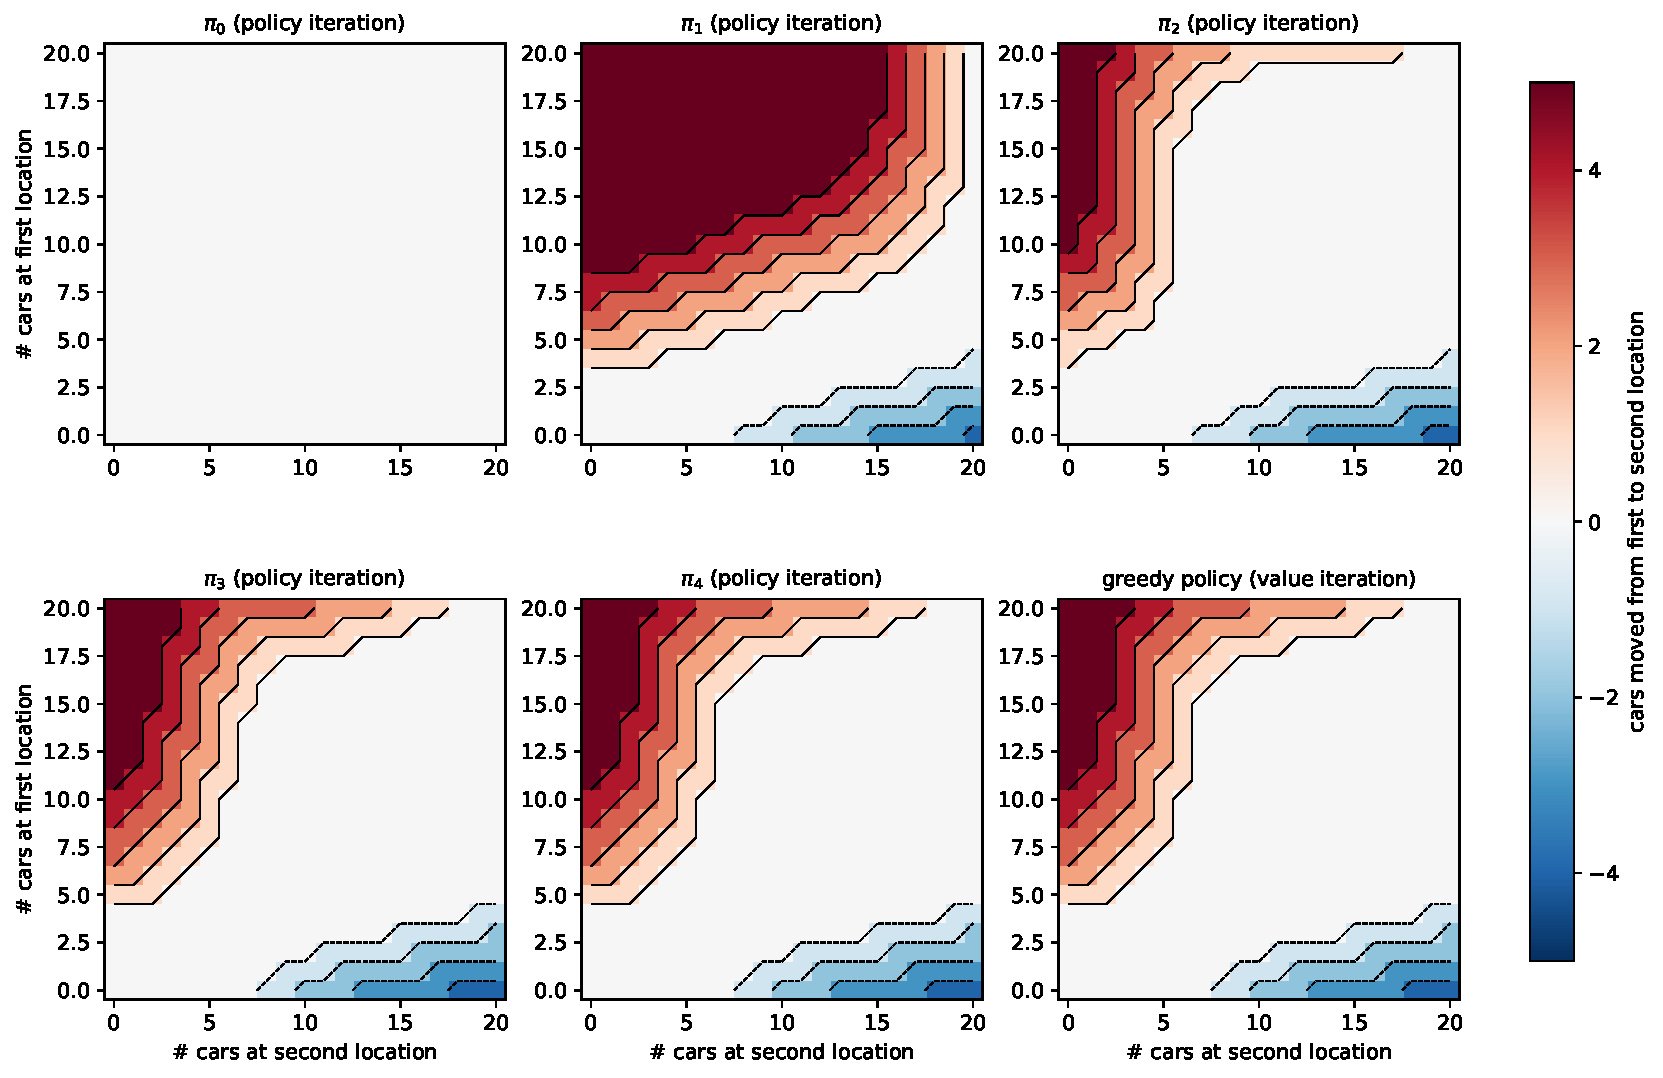
\includegraphics[width=\textwidth]{figures/jack_policies.pdf}
\caption{Policies $\pi_0, \dots, \pi_4$ found by policy iteration, and the greedy policy from value iteration. Positive numbers move cars from the first location to the second.}
\end{figure}

\begin{figure}[H]
\centering
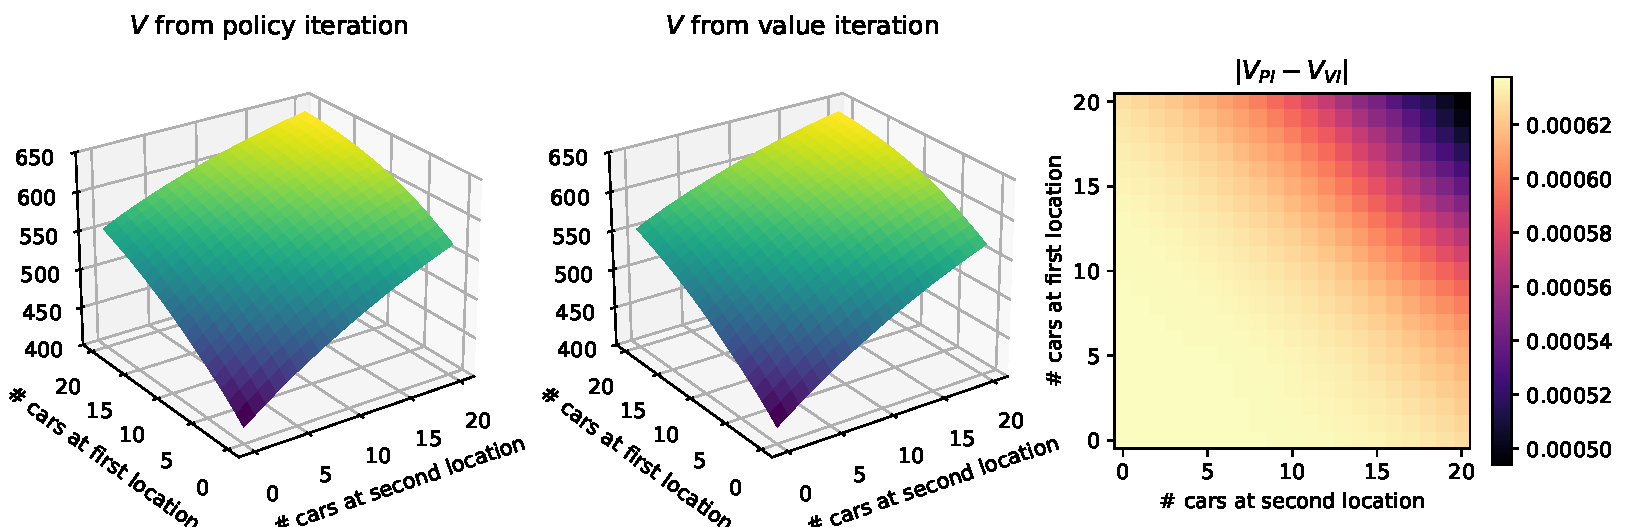
\includegraphics[width=\textwidth]{figures/jack_values.pdf}
\caption{Value functions computed by policy iteration and value iteration, and their difference.}
\end{figure}

\textbf{Results.}
\begin{itemize}
  \item \textbf{The two methods agree.} The largest difference between the two value functions is $6.4 \times 10^{-4}$, consistent with the stopping threshold, and the two policies are identical in all 441 states. The policies $\pi_1, \dots, \pi_4$ and the final value function have the same shape as in Figure 4.2.
  \item \textbf{Value range.} $V$ goes from $421$ at $(0, 0)$ to $637$ at $(20, 20)$. The minimum matches the figure, but the maximum is above the figure's top label of 612. The difference comes from the Poisson tails: if requests and returns of 11 or more are ignored, as in many implementations, the values drop to the range $[406, 618]$ (last cell of Exercise 2 in the notebook).
  \item \textbf{Iterations.} Policy iteration stops after 5 evaluations: the policy changes 4 times ($\pi_0 \to \pi_4$) and $\pi_4$ is stable. The evaluations take $126, 91, 80, 45, 14$ sweeps, 356 in total; they get shorter because each one starts from the previous $V$. Value iteration takes 126 sweeps.
  \item \textbf{Computational time.} With the vectorized implementation (median of 20 runs), policy iteration takes about $3.2$ ms and value iteration about $9.6$ ms. Policy iteration uses more sweeps, but an evaluation sweep only computes the value of the current action in each state (about $18\,\mu$s), while a value-iteration sweep computes all 11 actions and takes the maximum (about $71\,\mu$s). Policy iteration also needs only 5 improvement steps of that cost. So policy iteration is about 3 times faster here, although value iteration needs fewer sweeps.
\end{itemize}

\section*{Exercise 3: Policy iteration and value iteration with $Q$}

I write the dynamics as $p(s', r \mid s, a)$ with discount $\gamma$, and set $Q(s, a) = 0$ for terminal $s$. Using $V^\pi(s') = \sum_{a'} \pi(a' \mid s') Q^\pi(s', a')$ and $V^*(s') = \max_{a'} Q^*(s', a')$, the Bellman equations can be written with $Q$ only:
\begin{align*}
Q^\pi(s, a) &= \sum_{s', r} p(s', r \mid s, a) \Big[ r + \gamma \sum_{a'} \pi(a' \mid s')\, Q^\pi(s', a') \Big], \\
Q^*(s, a) &= \sum_{s', r} p(s', r \mid s, a) \Big[ r + \gamma \max_{a'} Q^*(s', a') \Big].
\end{align*}
Algorithms 2 and 3 apply these equations as updates.

\begin{algorithm}[tbp]
\caption{Policy iteration with $Q$ (estimates $\pi \approx \pi^*$)}
\begin{algorithmic}[1]
\Require threshold $\theta > 0$
\State initialize $Q(s, a)$ arbitrarily for all $s, a$, with $Q(s, \cdot) = 0$ for terminal $s$
\State initialize a deterministic policy $\pi(s) \in \mathcal{A}(s)$ arbitrarily
\Loop
  \State \textit{// Policy evaluation}
  \Repeat
    \State $\Delta \gets 0$
    \For{each non-terminal $s$ and each $a \in \mathcal{A}(s)$}
      \State $q \gets Q(s, a)$
      \State $Q(s, a) \gets \sum_{s', r} p(s', r \mid s, a) \big[ r + \gamma\, Q(s', \pi(s')) \big]$
      \State $\Delta \gets \max(\Delta, |q - Q(s, a)|)$
    \EndFor
  \Until{$\Delta < \theta$}
  \State \textit{// Policy improvement}
  \State $\textit{stable} \gets \text{true}$
  \For{each non-terminal $s$}
    \State $b \gets \pi(s)$
    \State $\pi(s) \gets \argmax_a Q(s, a)$, keeping $b$ if it is among the maximizers
    \If{$\pi(s) \neq b$} $\textit{stable} \gets \text{false}$ \EndIf
  \EndFor
  \If{\textit{stable}} \Return $Q \approx Q^*$, $\pi \approx \pi^*$ \EndIf
\EndLoop
\end{algorithmic}
\end{algorithm}

\begin{algorithm}[tbp]
\caption{Value iteration with $Q$ (estimates $Q \approx Q^*$ and $\pi \approx \pi^*$)}
\begin{algorithmic}[1]
\Require threshold $\theta > 0$
\State initialize $Q(s, a)$ arbitrarily for all $s, a$, with $Q(s, \cdot) = 0$ for terminal $s$
\Repeat
  \State $\Delta \gets 0$
  \For{each non-terminal $s$ and each $a \in \mathcal{A}(s)$}
    \State $q \gets Q(s, a)$
    \State $Q(s, a) \gets \sum_{s', r} p(s', r \mid s, a) \big[ r + \gamma \max_{a'} Q(s', a') \big]$
    \State $\Delta \gets \max(\Delta, |q - Q(s, a)|)$
  \EndFor
\Until{$\Delta < \theta$}
\State \Return $Q$ and the greedy policy $\pi(s) = \argmax_a Q(s, a)$
\end{algorithmic}
\end{algorithm}

\textbf{Remarks.}
\begin{itemize}
  \item \textbf{Correctness.} For $\gamma < 1$, the evaluation update is the Bellman operator of $Q^\pi$ and the value-iteration update is the Bellman optimality operator, both $\gamma$-contractions in the sup norm, so the iterates converge to $Q^\pi$ and $Q^*$. The improvement step is the same as in the $V$ version, because the quantity maximized there, $\sum_{s', r} p(s', r \mid s, a)[r + \gamma V^\pi(s')]$, is exactly $Q^\pi(s, a)$. For an undiscounted episodic task such as Exercise 1, the policies must be proper, as discussed in 1.3.
  \item \textbf{No model in the improvement step.} With $Q$, the greedy step only needs $\argmax_a Q(s, a)$ and no longer uses $p$. This is why Monte Carlo control (Exercise 6) estimates $Q$ rather than $V$.
  \item \textbf{Cost.} A sweep updates $|\mathcal{S}||\mathcal{A}|$ entries instead of $|\mathcal{S}|$. In value iteration, computing $\max_{a'} Q(s', a')$ once per state at the start of a sweep keeps the cost of a sweep of order $|\mathcal{S}|^2 |\mathcal{A}|$, as in the $V$ version.
  \item \textbf{Check.} In the notebook I ran both algorithms on the gridworld of Exercise 1. $Q$-policy iteration stops after 2 iterations and $Q$-value iteration after 5 sweeps. Both give $\max_a Q(s, a) = V^*(s)$ exactly.
\end{itemize}

\section*{Exercise 4: Evaluating the uniform policy}

\subsection*{4.1 Iterative policy evaluation}

I start from $V_0 = 0$ and apply Algorithm 1's evaluation step with the uniform policy, updating all states synchronously at each sweep. Starting from $0$, the iterates have a simple meaning: $V_k(s) = -\E^\pi_s[\min(k, \tau)]$, so they decrease to $V^\pi$, and the error $V_k(s) - V^\pi(s) = \E^\pi_s[(\tau - k)^+]$ decays like $\rho^k$, where $\rho = 0.9364$ is the spectral radius of $P$ from 1.2. Exact convergence would take infinitely many sweeps, so the number of sweeps depends on the threshold $\theta$:
\begin{center}
\begin{tabular}{ccc}
\toprule
$\theta$ & sweeps & $\max_s |V(s) - V^\pi(s)|$ \\
\midrule
$10^{-2}$  & 76  & $1.4 \times 10^{-1}$ \\
$10^{-4}$  & 146 & $1.5 \times 10^{-3}$ \\
$10^{-6}$  & 216 & $1.5 \times 10^{-5}$ \\
$10^{-8}$  & 286 & $1.5 \times 10^{-7}$ \\
$10^{-10}$ & 356 & $1.5 \times 10^{-9}$ \\
\bottomrule
\end{tabular}
\end{center}
Each factor 100 in $\theta$ costs about 70 more sweeps, as predicted by $\log(0.01)/\log\rho = 70.1$. The final error is about $\theta \rho/(1 - \rho) \approx 15\theta$. With $\theta = 10^{-4}$, the evaluation converges in 146 sweeps. I use $\theta = 10^{-10}$ (356 sweeps) for the reference $V^\pi$ below; it matches the exact solution of 1.2.

\subsection*{4.2 Monte Carlo prediction}

Every reward is $-1$, so the return from time $t$ of an episode that ends at time $\tau$ is $G_t = -(\tau - t)$. For each state I keep the sum and the number of returns collected so far, and $V^k(s)$ is their ratio after episode $k$. States that have not been visited yet keep $V^k(s) = 0$. First-visit MC uses only the first visit to $s$ in each episode, while every-visit MC uses all of them. Actions always follow the uniform policy. With exploring starts, $S_0$ is uniform over the 14 non-terminal states.

Figure 3 shows the value functions after $K = 1000$ episodes, and Figure 4 (left) shows $\epsilon_k = \|V^\pi - V^k\|_\infty$ for the same run. One run is noisy, so Figure 4 (right) and the table below average $\epsilon_k$ over 30 independent runs with $K = 5000$.

\begin{figure}[H]
\centering
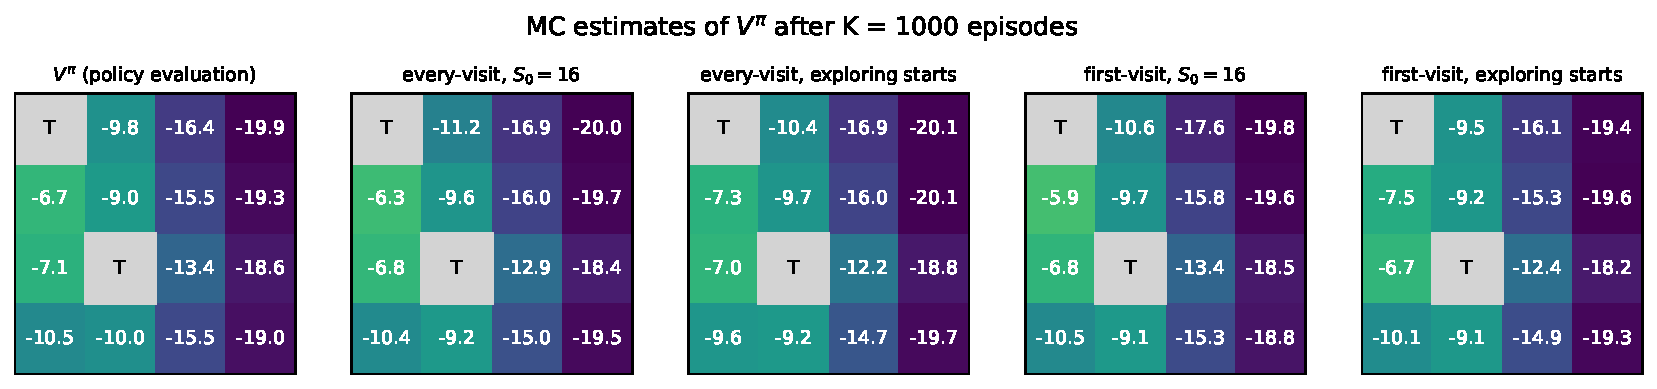
\includegraphics[width=\textwidth]{figures/mc_v_values.pdf}
\caption{$V^\pi$ from policy evaluation (left) and the four MC estimates after $K = 1000$ episodes.}
\end{figure}

\begin{figure}[H]
\centering
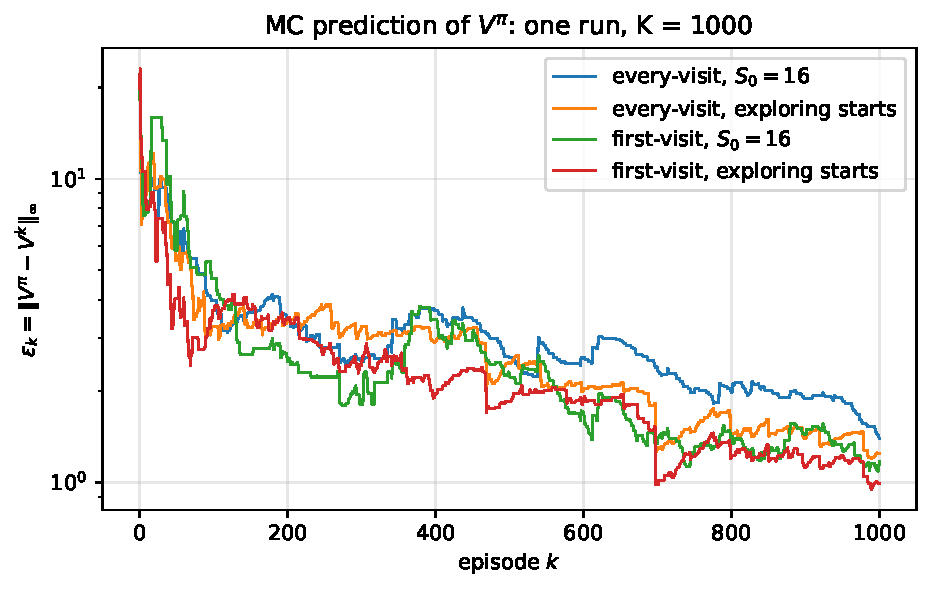
\includegraphics[width=0.49\textwidth]{figures/mc_v_errors.pdf}
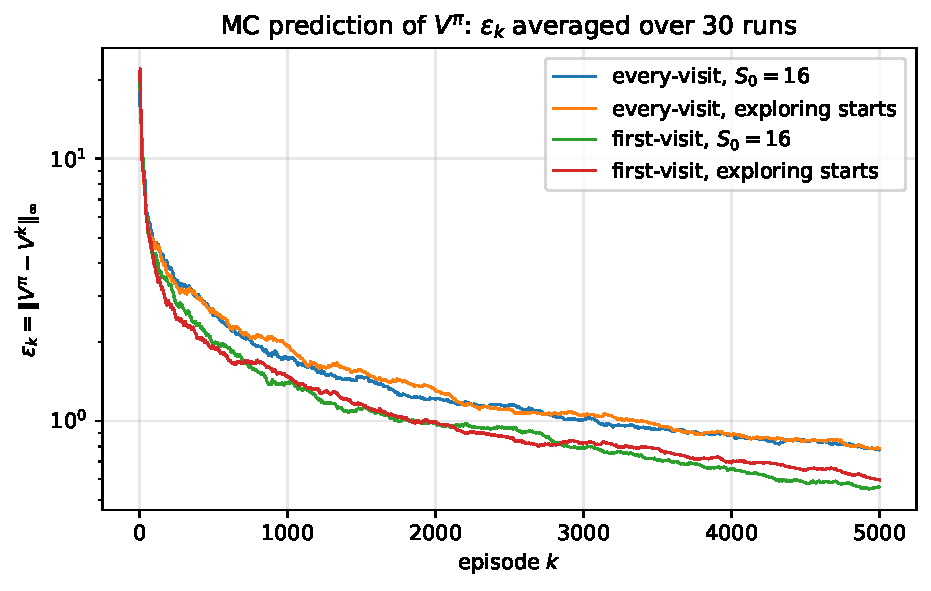
\includegraphics[width=0.49\textwidth]{figures/mc_v_errors_avg.pdf}
\caption{$\epsilon_k = \|V^\pi - V^k\|_\infty$ (log scale). Left: one run with $K = 1000$. Right: average over 30 runs with $K = 5000$.}
\end{figure}

\begin{center}
\begin{tabular}{lcccc}
\toprule
 & $\epsilon_{1000}$ (one run) & \multicolumn{3}{c}{average $\epsilon_k$ over 30 runs} \\
\cmidrule(lr){3-5}
Algorithm & & $k = 100$ & $k = 1000$ & $k = 5000$ \\
\midrule
every-visit, $S_0 = 16$        & 1.40 & 4.75 & 1.73 & 0.78 \\
every-visit, exploring starts  & 1.25 & 4.61 & 1.93 & 0.79 \\
first-visit, $S_0 = 16$        & 1.17 & 4.17 & 1.40 & 0.56 \\
first-visit, exploring starts  & 1.00 & 4.05 & 1.48 & 0.60 \\
\bottomrule
\end{tabular}
\end{center}

\textbf{Which algorithm converges faster?} First-visit MC converges faster than every-visit MC, with either start distribution: after 5000 episodes its average error is about $0.56$--$0.60$, compared with $0.78$--$0.79$. The start distribution matters much less. Exploring starts is slightly better during the first few hundred episodes, because all states are visited early, and $S_0 = 16$ is slightly better afterwards. In all cases the error decreases slowly, roughly like $1/\sqrt{k}$.

To explain this, I estimated by simulation (50{,}000 episodes) the variance constant of each estimator, i.e.\ the number $\sigma^2(s)$ such that the variance of $V^k(s)$ is about $\sigma^2(s)/k$:
\[
\sigma^2_{\text{first}}(s) = \frac{\E\big[(G_{\text{first}} - V^\pi(s))^2\, \1_{\text{visit}}\big]}{\pr(\text{visit})^2},
\qquad
\sigma^2_{\text{every}}(s) = \frac{\E\Big[\big(\sum_j (G_{t_j} - V^\pi(s))\big)^2\Big]}{\E[N_s]^2},
\]
where $t_j$ are the visit times and $N_s$ is the number of visits; the every-visit estimate is a ratio of sums over episodes.
\begin{center}
\small
\begin{tabular}{c ccc ccc}
\toprule
 & \multicolumn{3}{c}{$S_0 = 16$} & \multicolumn{3}{c}{exploring starts} \\
\cmidrule(lr){2-4} \cmidrule(lr){5-7}
$s$ & $\pr(\text{visit})$ & $\sigma^2_{\text{first}}$ & $\sigma^2_{\text{every}}$ & $\pr(\text{visit})$ & $\sigma^2_{\text{first}}$ & $\sigma^2_{\text{every}}$ \\
\midrule
2  & 0.24 & 723 & 1062 & 0.34 & 534 & 806 \\
3  & 0.31 & 727 & 1140 & 0.37 & 658 & 1092 \\
4  & 0.29 & 808 & 1437 & 0.31 & 816 & 1588 \\
5  & 0.15 & 685 & 1071 & 0.26 & 360 & 499 \\
6  & 0.30 & 515 & 892  & 0.40 & 400 & 558 \\
7  & 0.48 & 463 & 734  & 0.46 & 519 & 831 \\
8  & 0.47 & 499 & 790  & 0.38 & 664 & 1302 \\
9  & 0.15 & 622 & 859  & 0.25 & 388 & 528 \\
11 & 0.73 & 304 & 427  & 0.47 & 498 & 730 \\
12 & 0.74 & 322 & 483  & 0.39 & 660 & 1216 \\
13 & 0.19 & 662 & 1069 & 0.23 & 594 & 989 \\
14 & 0.44 & 358 & 586  & 0.32 & 522 & 768 \\
15 & 0.77 & 281 & 486  & 0.37 & 628 & 1040 \\
16 & 1.00 & 232 & 372  & 0.31 & 808 & 1437 \\
\bottomrule
\end{tabular}
\end{center}
\begin{itemize}
  \item \textbf{First-visit vs every-visit.} In every state, $\sigma^2_{\text{every}}$ is 1.4 to 2 times larger than $\sigma^2_{\text{first}}$. The returns from successive visits in the same episode share the same future, so they are strongly correlated, and the extra visits add little information. Moreover, every-visit gives more weight to episodes that come back to $s$ many times. These are the long episodes, whose returns are far from $V^\pi(s)$. Every-visit is also biased for finite $k$, while first-visit is unbiased.
  \item \textbf{$S_0 = 16$ vs exploring starts.} $\epsilon_k$ is a maximum over states, so the worst state matters. With $S_0 = 16$ the worst states are those far from 16 (2--5, 9, 13), which are visited in only 15--30\% of the episodes. With exploring starts the worst states are those far from the terminal states (4, 8, 12, 16), whose returns vary the most. In both cases the largest $\sigma^2_{\text{first}}$ is about 810, so the two start distributions give almost the same error. Exploring starts does not help much here because the uniform policy already explores the whole grid from state 16: an episode from 16 lasts 19 steps on average.
\end{itemize}

\section*{Exercise 5 (bonus): Estimating $Q^\pi$}

I now average the returns that follow each pair $(s, a)$, again with $G_t = -(\tau - t)$; first-visit uses the first occurrence of the pair in the episode. After episode $k$, I compute
\[
V^k(s) = \sum_a \pi(a \mid s)\, Q^k(s, a) = \frac{1}{4} \sum_a Q^k(s, a),
\]
with $Q^k(s, a) = 0$ for pairs that have not been visited yet. Since $\pi$ is uniform, the first action is already random, so exploring starts only needs a uniform $S_0$.

\begin{figure}[H]
\centering
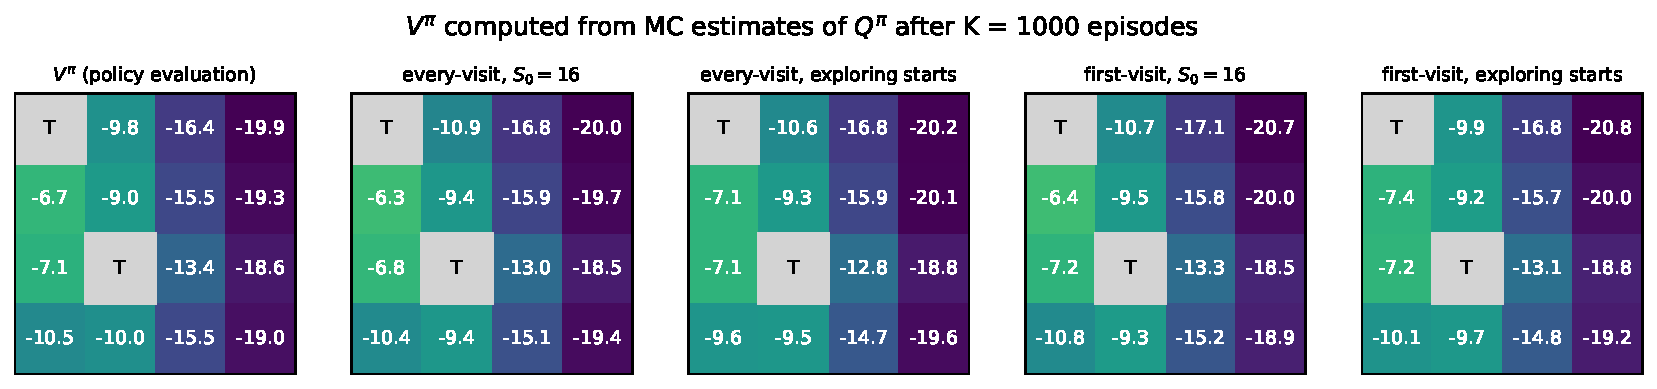
\includegraphics[width=\textwidth]{figures/mc_q_values.pdf}
\caption{$V^\pi$ from policy evaluation (left) and $V^k$ computed from the four MC estimates of $Q^\pi$ after $K = 1000$ episodes.}
\end{figure}

\begin{figure}[H]
\centering
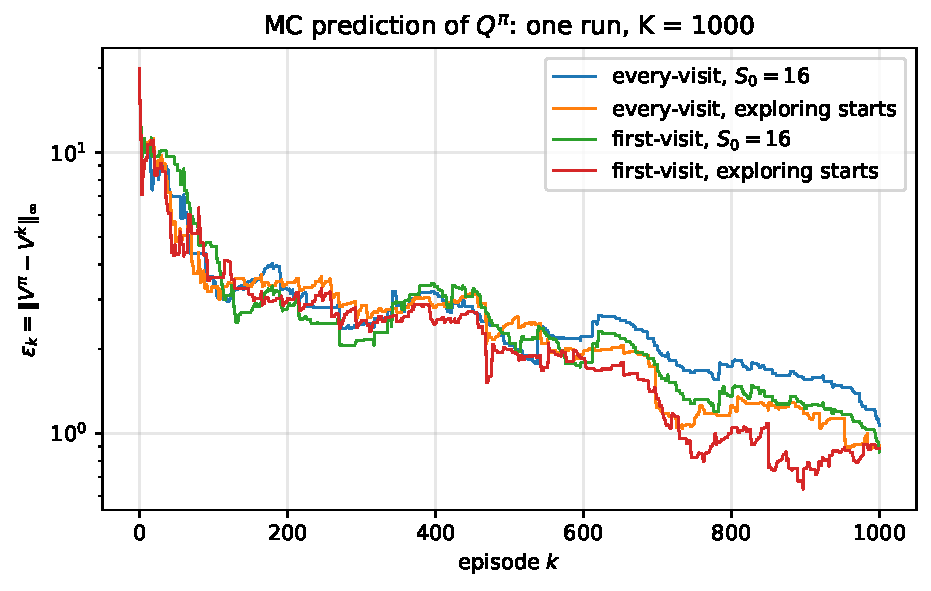
\includegraphics[width=0.49\textwidth]{figures/mc_q_errors.pdf}
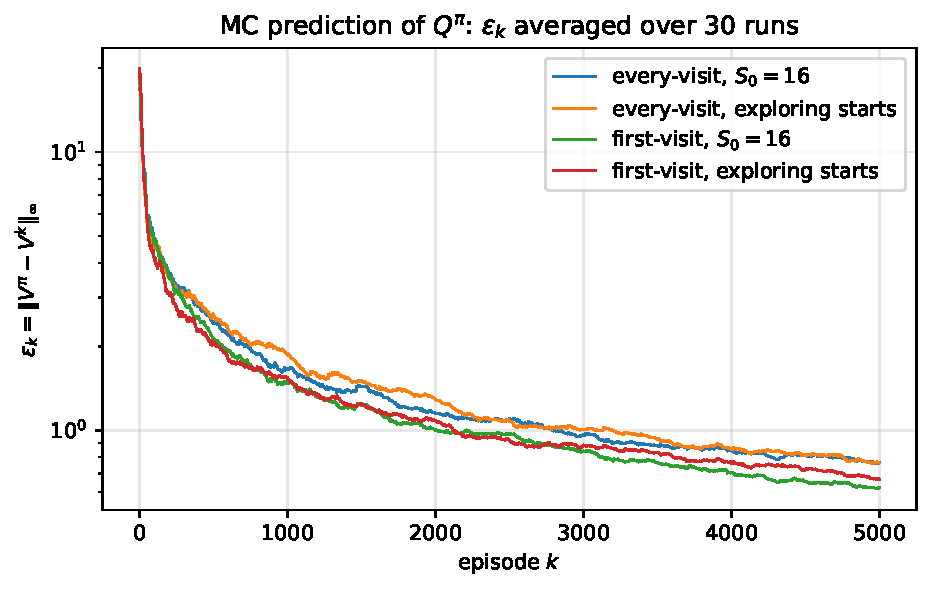
\includegraphics[width=0.49\textwidth]{figures/mc_q_errors_avg.pdf}
\caption{$\epsilon_k$ when $V^k$ is computed from $Q^k$. Left: one run with $K = 1000$. Right: average over 30 runs with $K = 5000$.}
\end{figure}

\begin{center}
\begin{tabular}{lccc}
\toprule
Average $\epsilon_k$ over 30 runs & $k = 100$ & $k = 1000$ & $k = 5000$ \\
\midrule
every-visit, $S_0 = 16$        & 4.80 & 1.66 & 0.77 \\
every-visit, exploring starts  & 4.60 & 1.87 & 0.76 \\
first-visit, $S_0 = 16$        & 4.74 & 1.48 & 0.62 \\
first-visit, exploring starts  & 4.18 & 1.53 & 0.67 \\
\bottomrule
\end{tabular}
\end{center}

The conclusions are the same as in Exercise 4: first-visit converges faster than every-visit, and the start distribution matters little. The every-visit errors are almost unchanged. First-visit is a bit worse than for $V^\pi$ ($0.62$ vs $0.56$ with $S_0 = 16$). This is consistent with the explanation above: a state can now contribute up to four returns per episode (the first visit of each action), and these are correlated in the same way as in every-visit MC.

\section*{Exercise 6 (bonus): Monte Carlo policy iteration}

I keep the improvement step of policy iteration and replace the exact evaluation by first-visit MC estimation of $Q^\pi$ from Exercise 5.

\begin{algorithm}[H]
\caption{Monte Carlo policy iteration}
\begin{algorithmic}[1]
\Require number of episodes $M$ per evaluation, maximal episode length $H$
\State $\pi \gets$ uniform policy
\Loop
  \State \textit{// MC policy evaluation (first-visit, exploring starts on $(S_0, A_0)$)}
  \State $\textit{Sum}(s, a) \gets 0$, $\textit{Count}(s, a) \gets 0$ for all $s, a$
  \For{$i = 1, \dots, M$}
    \State draw $(S_0, A_0)$ uniformly over non-terminal states $\times$ actions
    \State generate an episode $S_0, A_0, S_1, A_1, \dots$ with $A_t \sim \pi(\cdot \mid S_t)$ for $t \ge 1$, stopped at a terminal state or after $H$ steps
    \For{each pair $(s, a)$ visited, at its first visit $t$}
      \State $\textit{Sum}(s, a) \mathrel{+}= G_t$, $\textit{Count}(s, a) \mathrel{+}= 1$
    \EndFor
  \EndFor
  \State $Q(s, a) \gets \textit{Sum}(s, a) / \textit{Count}(s, a)$
  \State \textit{// Policy improvement (same as before)}
  \State $\pi_{\text{new}}(s) \gets \argmax_a Q(s, a)$ for each non-terminal $s$, keeping the old action on ties
  \If{$\pi_{\text{new}} = \pi$} \Return $\pi$, $Q$ \EndIf
  \State $\pi \gets \pi_{\text{new}}$
\EndLoop
\end{algorithmic}
\end{algorithm}

Two details matter:
\begin{itemize}
  \item \textbf{Exploring starts on $(S_0, A_0)$.} After the first improvement the policy is deterministic. Without a random first action, $Q(s, a)$ would never be estimated for $a \neq \pi(s)$, and the improvement step could not change the policy.
  \item \textbf{Episodes cut after $H$ steps.} A deterministic policy can loop forever, as in 1.1. A cut episode has a return of about $-H$, so the looping action looks very bad and is replaced at the next improvement. I use $M = 2000$ and $H = 200$.
\end{itemize}

\textbf{Results.} The algorithm stops after 2 iterations. The first evaluation estimates $Q^\pi$ for the uniform policy, and the greedy policy is already the optimal policy of 1.4. In the second evaluation the policy and the environment are deterministic, so after the random first action every return is exact. The estimate is then $Q^{\pi^*}$, and the policy is stable. The values $Q(s, \pi(s))$ are exactly $V^*$ from 1.4. I repeated the run with 20 random seeds, and every run found an optimal policy in 2 iterations.

\end{document}
